%%%%%%%%%%%%%%%%%%%%%%%%%%%%% Define Exam %%%%%%%%%%%%%%%%%%%%%%%%%%%%%%%%%%
\documentclass[addpoints]{exam}
%%%%%%%%%%%%%%%%%%%%%%%%%%%%%%%%%%%%%%%%%%%%%%%%%%%%%%%%%%%%%%%%%%%%%%%%%%%%%%%

%%%%%%%%%%%%%%%%%%%%%%%%%%%%% Using Packages %%%%%%%%%%%%%%%%%%%%%%%%%%%%%%%%%%
\usepackage{amsmath, amssymb, amsthm, amsfonts, geometry, venndiagram, tikz}
\usepackage{graphicx, xcolor, color, wrapfig, parskip, float, tabularx}
\usepackage[breaklinks]{hyperref}
\usepackage{colortbl, caption}
\usepackage{listings, mdframed, subfig, matlab-prettifier, hyperref}
\usepackage{lipsum, bookmark, booktabs, empheq, titlesec, verbatim, subfig, pdfpages, comment}
%%%%%%%%%%%%%%%%%%%%%%%%%%%%%%%%%%%%%%%%%%%%%%%%%%%%%%%%%%%%%%%%%%%%%%%%%%%%%%%
\definecolor{codebackground}{rgb}{0.95,0.95,0.95}
\definecolor{codegray}{rgb}{0.5,0.5,0.5}
\definecolor{codepurple}{rgb}{0.58,0,0.82}
\definecolor{codeblue}{rgb}{0.13,0.29,0.53}
\definecolor{ocre}{RGB}{243,102,25}
\definecolor{mygray}{RGB}{243,243,244}
\definecolor{deepGreen}{RGB}{26,111,0}
\definecolor{shallowGreen}{RGB}{235,255,255}
\definecolor{deepBlue}{RGB}{61,124,222}
\definecolor{shallowBlue}{RGB}{235,249,255}
\definecolor{softgray}{rgb}{0.95, 0.95, 0.95}
\definecolor{codegreen}{rgb}{0,0.6,0}
\definecolor{codegray}{rgb}{0.5,0.5,0.5}
\definecolor{codepurple}{rgb}{0.58,0,0.82}
\definecolor{backcolour}{rgb}{0.95,0.95,0.92}

%Code listing style named "mystyle"
\lstdefinestyle{mystyle}{
  backgroundcolor=\color{backcolour}, commentstyle=\color{codegreen},
  keywordstyle=\color{magenta},
  numberstyle=\tiny\color{codegray},
  stringstyle=\color{codepurple},
  basicstyle=\ttfamily\footnotesize,
  breakatwhitespace=false,         
  breaklines=true,                 
  captionpos=b,                    
  keepspaces=true,                 
  numbers=left,                    
  numbersep=5pt,                  
  showspaces=false,                
  showstringspaces=false,
  showtabs=false,                  
  tabsize=2
}

%"mystyle" code listing set
\lstset{style=mystyle}

\usetikzlibrary{arrows,shapes,positioning,shadows,trees}

%%%%%%%%%%%%%%%%%%%%%%%%%%%%% Header and Footer %%%%%%%%%%%%%%%%%%%%%%%%%%%%%%%%%%
\pagestyle{headandfoot}
\runningheadrule
\runningfootrule
\runningheader{Algorithms: Design and Analysis}{Weekly Challenge 02}{CS 412}
\runningfooter{}{Page \thepage\ of \numpages}{}
\firstpageheader{}{}{}
%%%%%%%%%%%%%%%%%%%%%%%%%%%%%%%%%%%%%%%%%%%%%%%%%%%%%%%%%%%%%%%%%%%%%%%%%%%%%%%

% Other Settings
% \boxedpoints
\printanswers
\qformat{}  %Comment this to number questions, uncomment this to not number questions

\newcommand\union\cup
\newcommand\inter\cap

%%%%%%%%%%%%%%%%%%%%%%%%%%%%%%% Title & Author %%%%%%%%%%%%%%%%%%%%%%%%%%%%%%%%

\title{Algorithms: Design and Analysis - CS 412 \vspace*{-4mm}}
\author{Weekly Challenge 02: Sorting}
\date{\vspace*{-4mm} Ali Muhammad Asad - aa07190}

% \pgfplotsset{compat=1.18}

%%%%%%%%%%%%%%%%%%%%%%%%%%%%%%%%%%%%%%%%%%%%%%%%%%%%%%%%%%%%%%%%%%%%%%%%%%%%%%%

\begin{document}
\maketitle

% {\small \begin{center} \gradetable[h] \end{center}}

\begin{questions}
  \question[1]
  \textbf{1.}\; (1 point) A decision tree is a binary tree that represents the comparisons between elements that are performed by a particular sorting algorithm operating on an input of a given size. Control, data movement, and all other aspects of the algorithm are ignored. The leaf nodes represent all possible permutations (arrangements) of the input array. For example, the following is a decision tree of the bubble sort algorithm for $n = 3$, where $n$ is the total number of elements in an array.
  \begin{figure}[htbp]
    \centering
    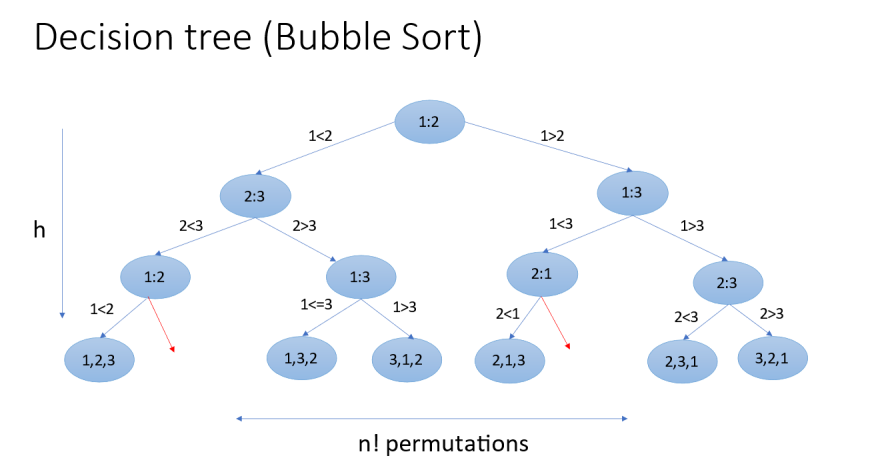
\includegraphics[width=\textwidth]{dtree.png}
  \end{figure}

  Take $n = 3$,  and compare the efficiency of selection sort and insertion sort, in terms of the number of comparisons, with the help of a decision tree when the array is: \begin{enumerate}
    \item Fully sorted
    \item Fully unsorted
  \end{enumerate}

  Please draw the decision tree for both algorithms and give your analysis in three to four lines.

  \begin{solution}
    Selection sort works by repeatedly finding the minimum element from the unsorted array, and putting it at at the beginning, thus dividing the array into two groups; the sorted subarray and the unsorted subarray. The decision tree for selection sort for 3 arbitrary elements $ \{ a, b, c \} $ is shown below:
    \begin{figure}[H]
      \centering
      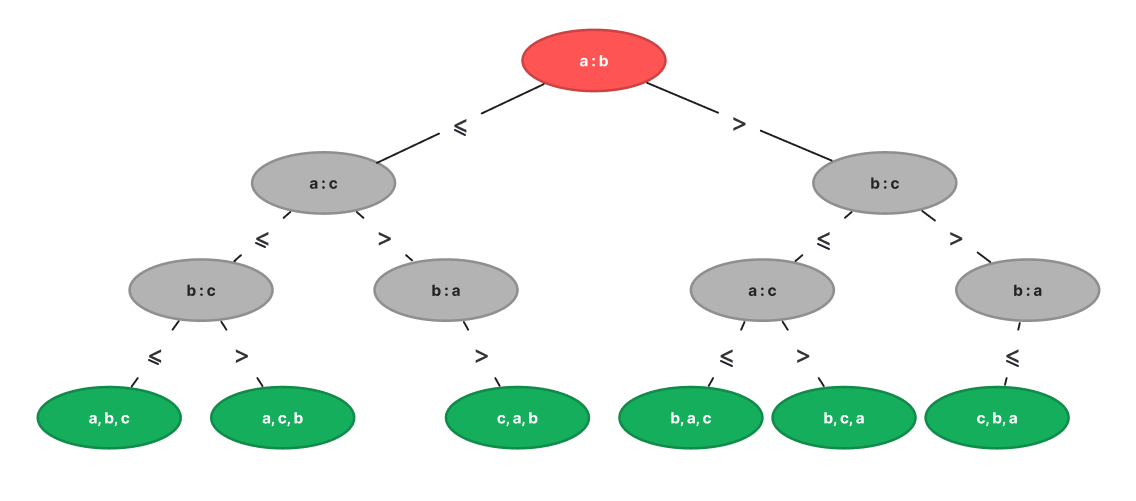
\includegraphics[width=\textwidth]{selection.png}
      \caption{Decision tree for selection sort}
    \end{figure}

    Insertion sort works by repeatedly inserting the next element from the unsorted subarray into the sorted subarray. The decision tree for insertion sort for 3 arbitrary elements $ \{ a, b, c \} $ is shown below:
    \begin{figure}[H]
      \centering
      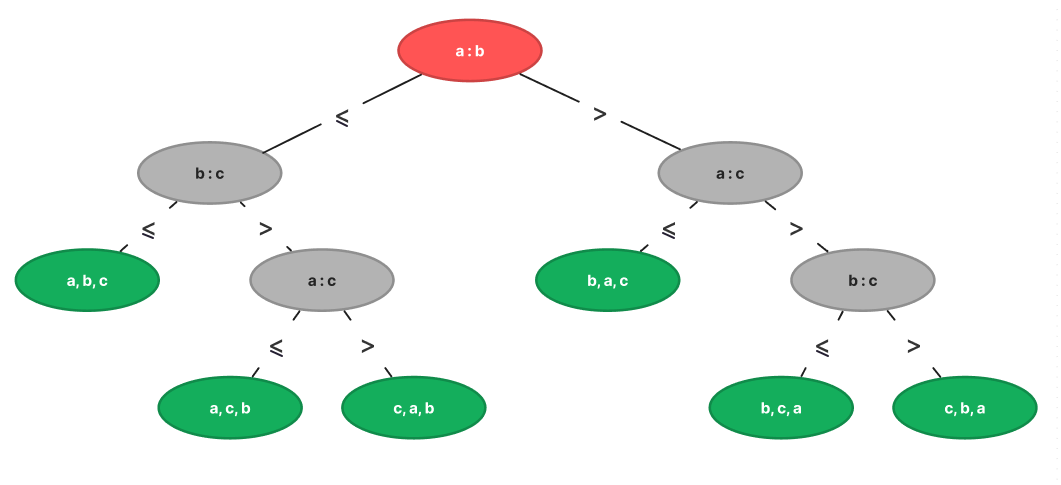
\includegraphics[width=\textwidth]{insertion.png}
      \caption{Decision tree for insertion sort}
    \end{figure}

    In both the above figures, the \textcolor{red}{red node} represents the root node, the \textcolor{deepGreen}{green nodes} represent the leaf nodes (which are also the possible permutations of our elements), while the other nodes are the intermediary nodes.

    \begin{enumerate}
      \item \textbf{Fully sorted:} \begin{itemize}
        \item Selection Sort: there are 3 comparisons for the fully sorted array, since selection sort works by comparing each element to the rest of the elements in the array, and then swapping the appropriate elements. 
        \item Insertion Sort: there are 2 comparisons for the fully sorted array, since insertion sort compares each element first by its previous element. Therefore, when the array is fully sorted, excluding the first element, all elements are compared once.
      \end{itemize}
      \item \textbf{Fully unsorted:} \begin{itemize}
        \item Selection Sort: there are 3 comparisons for the fully unsorted array, by the same argument as above.
        \item Insertion Sort: there are 3 comparisons for the fully unsorted array, since insertion sort compares each element first by its previous element. Therefore, when the array is fully unsorted, all elements are compared.
      \end{itemize}
    \end{enumerate}

    While both algorithms have the same performance for the fully unsorted array, insertion sort is more efficient for the fully sorted array.
    
    In general, selection sort does $ \frac{n(n - 1)}{2} = O(n^2) $ comparisons in the best and worst case, while insertion sort does $ (n - 1) = O(n) $ comparisons in the best case and $ \frac{n(n - 1)}{2} = O(n^2) $ comparisons in the worst case.

  \end{solution}

\end{questions}

\end{document}